\chapter[Hierarchical Selective Classification]{Hierarchical Selective Classification of European Land Use / Land Cover using pixel-based uncertainty}
\label{cha:chapter4}
\vspace*{\fill}
This chapter is based on:
\\
\\
% Full citation of the published (or submitted/in review) article
% This refers to the article key in the refs.bib file.
\fullcite{witjes2024hierarchical}
\newpage

\section*{Abstract}
% HAS TO HAVE ALL SECTIONS

% CAN BE SHORT AND UNCOOKED

% SOME CLEAR RESULTS
\newpage

\section{Introduction}
[Land cover is important.]

\subsection{Land cover mapping}

    \subsection{Where do you get data?}

        It's important to use separate sets for training and validating models. The LUCAS points are the best available validations samples for Europe because they have a rigorous sampling design, cover a wide range of land cover classes, and include data from multiple years \citep{dandrimont2020harmonised,dandrimont2021lucas,venter2022global}. The CORINE Land Cover dataset is a useful source of training data \citep{witjes2022spatiotemporal,witjes2024iterative}, but it lacks many classes at the thematic depth of the LUCAS legend, especially regarding crop types.
        The EuroCrops dataset provides many of these classes at a level even more fine-grained than LUCAS itself \citep{schneider2023eurocrops}. Lastly, the volunteered geographical information of OpenStreetMap can be mined for land cover polygons \citep{witjes2022spatiotemporal}, especially if they relate to anthropogenic land cover types [CITE?]. 
        
    \subsection{Detail and accuracy}
        
        Mapping many classes is more difficult:
        \begin{enumerate}
        \item Collecting training and validation samples
        \item Model training (more confusion)
        \item Map interpretability (harder to read)
        \end{enumerate}
        It is not often done at high spatial resolution.

    \subsection{Prediction uncertainty}
        Prediction uncertainty = the chance that a specific prediction is correct.
        You can use heuristics but they don't give a statistical guarantee. Examples are the predicted probabilities, especially if they are well-calibrated \citep{niculescu2005predicting}, the margin of victory (the difference between the probabilities of the highest and second highest class) \citep{calderon2021high}, and model variance from ensembles of classifiers \citep{witjes2022spatiotemporal}. \citet{witjes2024iterative} found indications of a relationship between a prediction's certainty and the iteration at which it is classified by IMP.

    \subsection{Selective classification}
        Selective classification, also known as reject option classification, introduces a mechanism within classification models to abstain from making a prediction when the model's confidence is below a certain threshold. This approach aims to enhance the overall reliability and accuracy of the model by only making decisions when the model is sufficiently certain. \citet{geifman2017selective} emphasize the potential of selective classification in improving the safety and robustness of machine learning applications, particularly in critical areas such as medical diagnosis and autonomous driving. By implementing a reject option, models can effectively reduce the risk of making incorrect predictions at the cost of not making a decision in all cases. This trade-off is particularly crucial in scenarios where the cost of an error far outweighs the benefit of a correct but uncertain prediction. The selective classification framework thus provides a pragmatic approach to managing uncertainty and enhancing decision quality in machine learning systems.

    \subsection{Hierarchical classification}
        \citet{kim2016modis} leveraged a small hierarchical legend by using different models to identify sub-classes of different crop types. A similar approach was tried with the Brazilian PRODES project, where first a forest mask was created with high precision (user's accuracy); subsequent forest change detection algorithms were later only applied to the area covered by the forest mask \citep{hansen2008comparing}.

    \subsection{Research gaps}
        It is likely that prediction uncertainty will be higher when there are more classes in a legend, especially when they are spectrally similar, such as different cereal types. This introduces errors in the map that could be avoided by having a simpler legend, but this sacrifices thematic depth for accuracy There is a need for maps that are more detailed than the typical 'artificial, forest, cropland, grasland, water' type classes, so navigating the trade-off between accuracy and detail must be done.

    \subsection{This paper}
        In this paper, we demonstrate an improved version of the framework proposed by \citep{witjes2022spatiotemporal} to extract training data from multiple open land cover polygon datasets (Eurocrops, OpenStreetmap, and Corine Land Cover) from several years across Europe. 
        
        We train a land cover classification model and predict probabilities for 53 LUCAS land cover classes.
        
        We create hard-class maps using maximum probability assignment and Iterative Mapping of Probabilities (IMP) \citep{witjes2024iterative} for each level in the hierarchical legend, and then aggregate uncertain predictions to a higher level in the legend to minimize error. We compare three different uncertainty metrics: The highest predicted probability and margin of victory (difference between the highest and second highest), and the iteration at which a pixel was classified during IMP.
        
        Each metric is used to generate hard class maps where uncertain predictions are aggregated to more general classes (e.g. \textit{Rice} and \textit{Wheat} to \textit{Cereals}, and \textit{Cereals} and \textit{Root crops} to \textit{Cropland}). We validate the resulting hard class maps with LUCAS land cover observations, and assess how well each metric can be used to navigate the trade-off between accuracy and detail.

\section{Methods}

\begin{figure}[H]
    \centering
    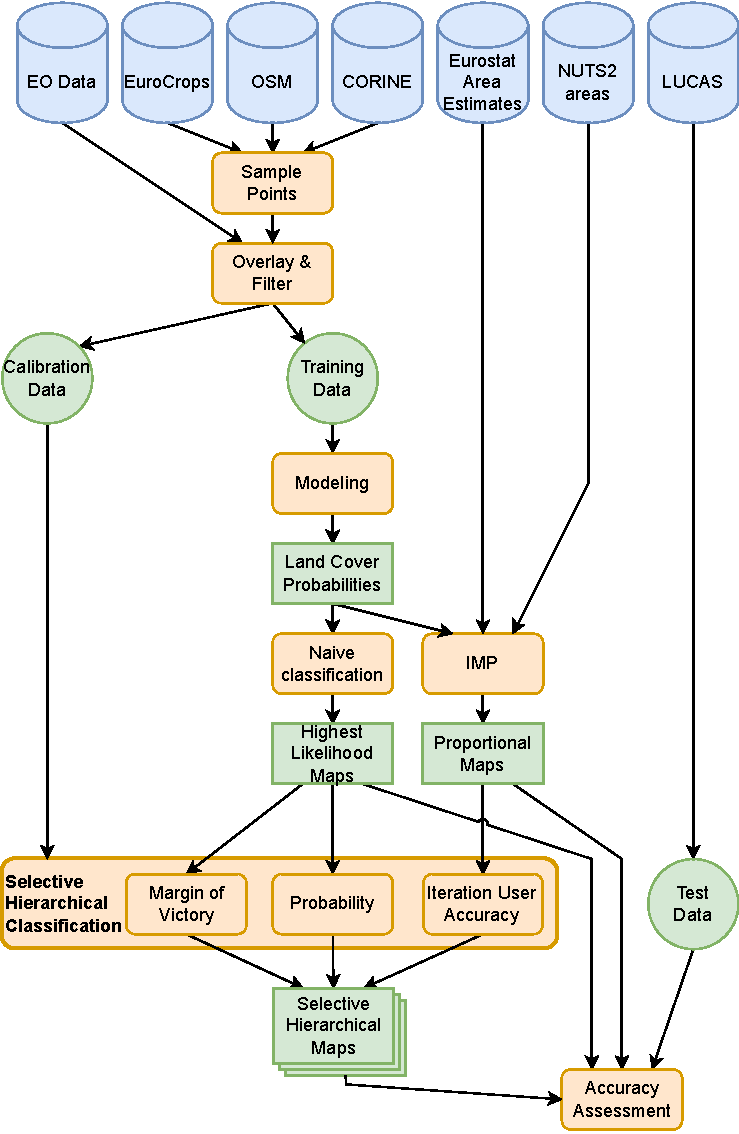
\includegraphics[width=\textwidth]{figs_05/fig_methodology.pdf}
    \caption{The methodology of this research.}
    \label{fig:05_methodology}
\end{figure}

\subsection{Selection of study area}

We obtained Nomenclature of Territorial Units for Statistics (NUTS) administrative boundaries from EuroStat. %https://ec.europa.eu/eurostat/web/gisco/geodata/reference-data/administrative-units-statistical-units/nuts
We matched level 2 NUTS areas to the earliest LUCAS survey since each update (See Table~\ref{tab:05_NUTS_LUCAS}). 

We selected all NUTS2 areas:
1. For which LUCAS land cover area estimates were available;
2. For which more than 500 LUCAS points were available;
2. Whose area was below the largest 1\% surface area among NUTS2 areas (to maintain computational feasibility)

We randomly selected up to four NUTS2 area/year combinations each country.

\begin{table}[H]
    \centering
    \begin{tabular}{c|c}
         NUTS update year &  LUCAS survey year\\
         2006 & 2006 \\
         2010 & 2012 \\
         2013 & 2015 \\
         2016 & 2018 \\
    \end{tabular}
    \caption{Caption}
    \label{tab:05_NUTS_LUCAS}
\end{table}

\subsection{Legend harmonization}
% https://docs.google.com/spreadsheets/d/1UJrbdGJgrXlW_WnSoDVIhf68dz8XoiWrZW6WVeR5lPw/edit#gid=1654270911
For some classes, either no area estimates or no training data was found. This required us to merge some classes, and aggregate others to a higher level in the hierarchical legend. Table \ref{tab:05_legend_harmonization} shows which LUCAS classes were aggregated and merged, and for what reason.


\begin{table}[]
% https://docs.google.com/spreadsheets/d/1UJrbdGJgrXlW_WnSoDVIhf68dz8XoiWrZW6WVeR5lPw/edit#gid=213241018
\resizebox{0.8\textwidth}{!}{% Resize table to fit within page width

\begin{tabular}{llll}
\textbf{LUCAS land cover class}                        & \textbf{Training data source}   & \textbf{Used land cover class}                                 & \textbf{Reason for change}\\
A11: Buildings with one to three floors       & \multirow{2}{*}{corine} & \multirow{2}{*}{A10: Roofed built-up areas}           & No training data                                          \\
A12: Buildings with more than three floors    &                         &                                                       & No training data                                          \\
\multirow{2}{*}{A13: Greenhouses}             & openstreetmap           & \multirow{2}{*}{A13: Greenhouses}                     &                                                           \\
                                              & eurocrops               &                                                       &                                                           \\
A21: Non built-up area features               & \multirow{2}{*}{corine} & \multirow{2}{*}{A20: Artificial non-built up areas}   & No training data                                          \\
A22: Non built-up linear features             &                         &                                                       & No training data                                          \\
B11: Common wheat                             & eurocrops               & B11: Common wheat                                     &                                                           \\
B12: Durum wheat                              & eurocrops               & B12: Durum wheat                                      &                                                           \\
B13: Barley                                   & eurocrops               & B13: Barley                                           &                                                           \\
B14: Rye                                      & eurocrops               & B14: Rye                                              &                                                           \\
B15: Oats                                     & eurocrops               & B15: Oats                                             &                                                           \\
B16: Maize                                    & eurocrops               & B16: Maize                                            &                                                           \\
B17: Rice                                     & corine                  & B17: Rice                                             &                                                           \\
B17: Rice                                     & eurocrops               & B17: Rice                                             &                                                           \\
B18: Triticale                                & eurocrops               & B18: Triticale                                        &                                                           \\
B19: Other cereals                            & eurocrops               & \multirow{2}{*}{B19: Other cereals}                   &                                                           \\
B54: Mixed cereals for fodder                 &                         &                                                       & No training data                                          \\
B21: Potatoes                                 & eurocrops               & B21: Potatoes                                         &                                                           \\
B22: Sugar beet                               & eurocrops               & B22: Sugar beet                                       &                                                           \\
B23: Other root crops                         & eurocrops               & B23: Other root crops                                 &                                                           \\
B31: Sunflower                                & eurocrops               & B31: Sunflower                                        &                                                           \\
B32: Rape and turnip rape                     & eurocrops               & B32: Rape and turnip rape                             &                                                           \\
B33: Soya                                     & eurocrops               & B33: Soya                                             &                                                           \\
B34: Cotton                                   & eurocrops               & \multirow{2}{*}{B35: Other fibre and olaginous crops} & No training data\\
B35: Other fibre and olaginous crops          & eurocrops               &                                                       &                                                           \\
B36: Tobacco                                  & eurocrops               & B36: Tobacco                                          &                                                           \\
B37: Other non-permanent industrial crops     & eurocrops               & B37: Other non-permanent industrial crops             &                                                           \\
B41: Dry pulses                               & eurocrops               & B41: Dry pulses                                       &                                                           \\
B42: Tomatoes                                 & eurocrops               & B42: Tomatoes                                         &                                                           \\
B43: Other fresh vegetables                   & eurocrops               & B43: Other fresh vegetables                           &                                                           \\
B44: Floriculture and ornamental plants       & eurocrops               & B44: Floriculture and ornamental plants               &                                                           \\
B45: Strawberries                             & eurocrops               & B45: Strawberries                                     &                                                           \\
B51: Clovers                                  & eurocrops               & B51: Clovers                                          &                                                           \\
B52: Lucerne                                  & eurocrops               & B52: Lucerne                                          &                                                           \\
B53: Other leguminous and mixtures for fodder & eurocrops               & B53: Other leguminous and mixtures for fodder         &                                                           \\
B55: Temporary grasslands                     & eurocrops               & B55: Temporary grasslands                             &                                                           \\
B71: Apple fruit                              & eurocrops               & B71: Apple fruit                                      &                                                           \\
B72: Pear fruit                               & eurocrops               & B72: Pear fruit                                       &                                                           \\
B73: Cherry fruit                             & eurocrops               & B73: Cherry fruit                                     &                                                           \\
B74: Nuts trees                               & eurocrops               & B74: Nuts trees                                       &                                                           \\
B75: Other fruit trees and berries            & eurocrops               & B75: Other fruit trees and berries                    &                                                           \\
B76: Oranges                                  &                         & \multirow{2}{*}{B77: Other citrus fruit}              & No training data                                          \\
B77: Other citrus fruit                       & eurocrops               &                                                       &                                                           \\
\multirow{2}{*}{B81: Olive groves}            & corine                  & \multirow{2}{*}{B81: Olive groves}                    &                                                           \\
                                              & eurocrops               &                                                       &                                                           \\
\multirow{2}{*}{B82: Vineyards}               & corine                  & \multirow{2}{*}{B82: Vineyards}                       &                                                           \\
                                              & eurocrops               &                                                       &                                                           \\
B83: Nurseries                                & eurocrops               & B83: Nurseries                                        &                                                           \\
B84: Permanent industrial crops               & eurocrops               & B84: Permanent industrial crops                       &                                                           \\
C10: Broadleaved woodland                     & corine                  & C10: Broadleaved woodland                             &                                                           \\
C21: Spruce dominated coniferous woodland     & \multirow{3}{*}{corine} & \multirow{3}{*}{C20: Coniferous woodland}             & No area estimates                                         \\
C22: Pine dominated coniferous woodland       &                         &                                                       & No area estimates                                         \\
C23: Other coniferous woodland                &                         &                                                       & No area estimates                                         \\
C31: Spruce dominated mixed woodland          & \multirow{3}{*}{corine} & \multirow{3}{*}{C30: Mixed woodland}                  & No area estimates                                         \\
C32: Pine dominated mixed woodland            &                         &                                                       & No area estimates                                         \\
C33: Other mixed woodland                     &                         &                                                       & No area estimates                                         \\
D10: Shrubland with sparse tree cover         & corine                  & D10: Shrubland with sparse tree cover                 &                                                           \\
D20: Shrubland without tree cover             & corine                  & D20: Shrubland without tree cover                     &                                                           \\
E10: Grassland with sparse tree/shrub cover   &                         & \multirow{4}{*}{E00: Grassland}                       & No training data                                          \\
E20: Grassland without tree/shrub cover       & eurocrops               &                                                       & No area estimates                                         \\
E20: Grassland without tree/shrub cover       & corine                  &                                                       & No area estimates                                         \\
E30: Spontaneously re-vegetated surfaces      &                         &                                                       & No training data                                          \\
F10: Rocks and stones                         & \multirow{3}{*}{corine} & \multirow{3}{*}{F00: Bare land and lichens/moss}      & No area estimates                                         \\
F20: Sand                                     &                         &                                                       & No area estimates                                         \\
F40: Other bare soil                          &                         &                                                       & No area estimates                                         \\
G11: Inland fresh water bodies                & \multirow{8}{*}{corine} & \multirow{8}{*}{G00: Water areas}                     & No area estimates                                         \\
G12: Inland salty water bodies                &                         &                                                       & No area estimates                                         \\
G21: Inland fresh running water               &                         &                                                       & No area estimates                                         \\
G22: Inland salty running water               &                         &                                                       & No area estimates                                         \\
G30: Transitional water bodies                &                         &                                                       & No area estimates                                         \\
G30: Transitional water bodies                &                         &                                                       & No area estimates                                         \\
G40: Sea and ocean                            &                         &                                                       & No area estimates                                         \\
G50: Glaciers, permanent snow                 &                         &                                                       & No area estimates                                         \\
H11: Inland marshes                           & \multirow{5}{*}{corine} & H11: Inland marshes                                   &                                                           \\
H12: Peatbogs                                 &                         & H12: Peatbogs                                         &                                                           \\
H21: Salt marshes                             &                         & H21: Salt marshes                                     &                                                           \\
H22: Salines and other chemical deposits      &                         & H22: Salines and other chemical deposits              &                                                           \\
H23: Intertidal flats                         &                         & H23: Intertidal flats                                 &                                                          
\end{tabular}
}
\caption{Overview of LUCAS classes, and how they were aggregated to the legend used in this work. Each entry also shows which datasets were used to extract training data for the class, and why any aggregations were made. 'No training data' indicates that sources of unambiguous polygon data were not found, and 'No area estimates' means that Eurostat does not publish area estimates at the required thematic level.}
\label{tab:05_legend_harmonization}
\end{table}

\subsection{Training and Calibration Samples}
We extracted polygons from CORINE, EuroCrops and OpenStreetmap. Table~\ref{tab:05_legend_harmonization} shows the training data source per LUCAS class. We randomly sampled points from polygons. One point minimum, one extra point per 9 30m pixels of polygon surface, to a maximum of 20 points per polygon.
We filtered the samples with Copernicus HRL layers and OpenStreetmap building and roads data. Any sample that did not meet the following criteria was removed from the dataset.
\begin{enumerate}
    \item \textit{A10: Roofed built up areas} without buildings according to OSM or not impervious according to Copernicus Imperviousness
    \item \textit{A20: Artificial non-built up areas} with buildings or low Copernicus imperviousness
    \item Non-\textit{Artificial} classes with OSM buildings or high Copernicus imperviousness
    \item \textit{C00: Woodland} classes without Copernicus Tree Cover
    \item \textit{D10: Shrubland} with sparse tree cover with Copernicus Tree Cover below 1\% or above 75\%
    \item \textit{D20: Shrubland} without tree cover with Copernicus Tree Cover above 1\%.
    \item \textit{E00: Grassland} without Copernicus Grassland or with Copernicus Tree Cover above 10\%
    \item \textit{F00: Bare land} and lichens/moss with Copernicus Grass or Tree cover
    \item \textit{G00: Water areas} with Copernicus Grassland or Tree Cover
    \item Non-\textit{Water} classes with Copernicus Permanent Water
    \item \textit{H00: Wetlands} classes without Copernicus temporary wetness (excluding \textit{H23: Intertidal Flats})
\end{enumerate}

We split the polygon-sampled points into a training and calibration set with a 0.75/0.25 split.

\subsection{Land Cover Classification}
We trained a LightGBM gradient boosting model \citep{ke2017lightgbm} on the training samples.
We predicted land cover probabilities on calibration points for all 53 LUCAS land cover classes and derived hard class maps using maximum probability assignment. For each calibration point, we stored the probability of the assigned class and the margin of victory.
We then applied the IMP algorithm on the calibration points, using the class distribution of the calibration points as a proxy of the area estimate.

\section{Results}
    \subsection{Training data}

        We sampled ~41 million points from the CORINE, EuroCrops and OpenStreetmap polygons. The filtering procedure removed ~25\% of samples, resulting in a dataset of 32 million samples, which was split into 24 million training samples and 8 million calibration samples.
    
\subsection{Validation data}

    Sampling one combination of a NUTS2 area and LUCAS survey year per country yielded 25 regions. Iteratively adding more area/year combinations to guarantee at least 30 LUCAS points per class in the validation dataset resulted in 17 more, with 9 of them being added to guarantee coverage of \textit{Intertidal Flats}, 3 for \textit{Strawberries}, and 3 for \textit{Tobacco}. This resulted in a total of 52 areas with at least 300 LUCAS observations, containing a total of 66994 observations (See table \ref{tab:05_lucas_nuts}. Figure~\ref{fig:05_lucas_aoi} shows all areas that were selected.

    \begin{table}[H!]
    \begin{tabular}{lll}
    Year & NUTS2 areas & LUCAS points \\
    2012 & 7           & 7.468        \\
    2015 & 16          & 20.407       \\
    2018 & 29          & 39.119      
    \end{tabular}
    \caption{Sampled NUTS2 areas and LUCAS observations selected as validation data, separated per survey year.}
    \label{tab:05_lucas_nuts}
    \end{table}
    
    \begin{figure}[H!]
    \centering
    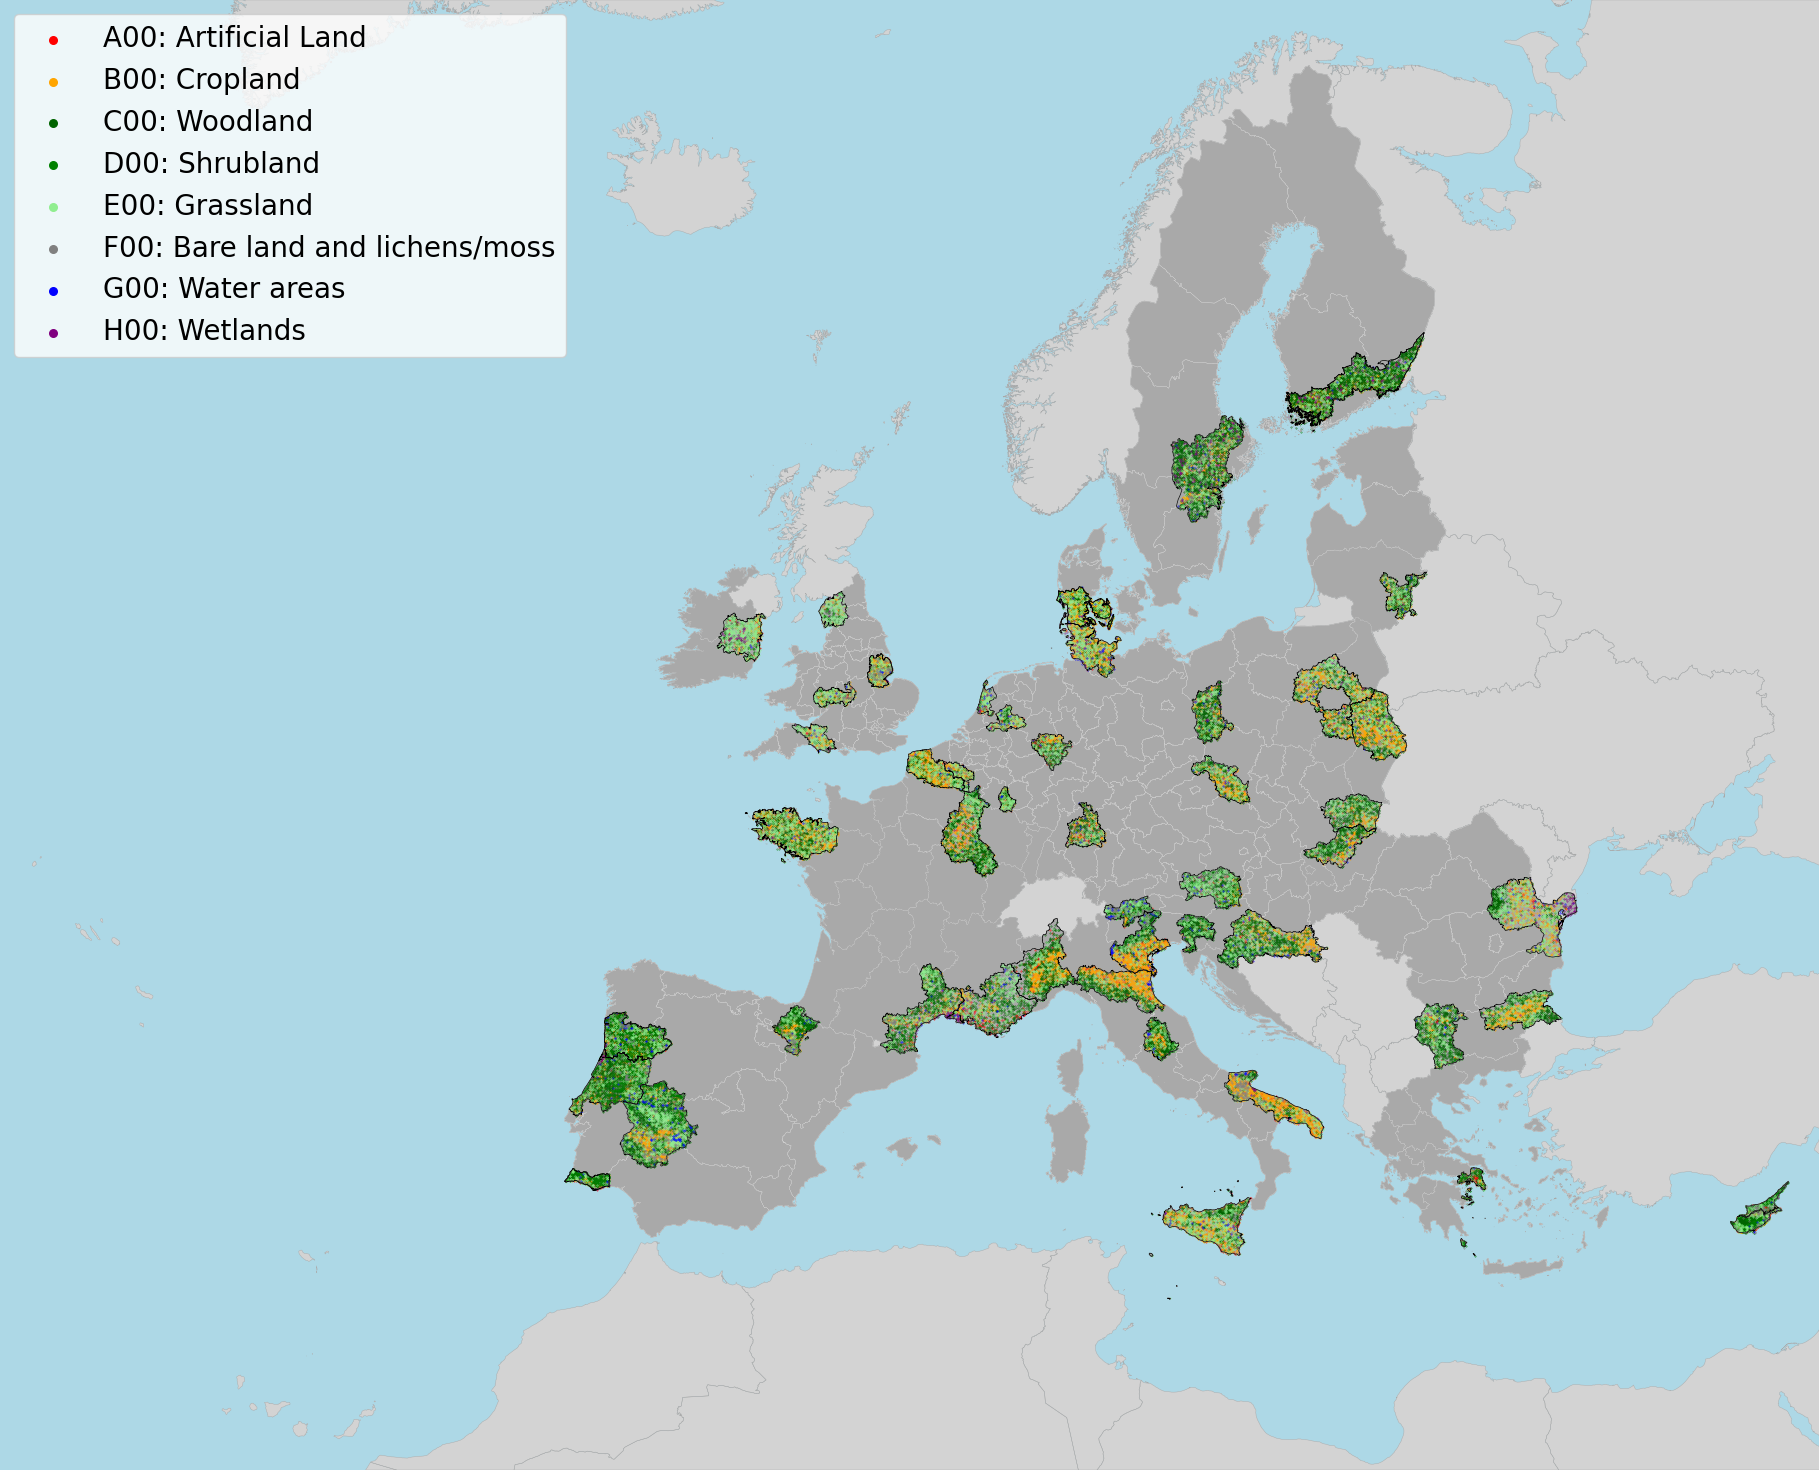
\includegraphics[width=\textwidth]{figs_05/fig_lucas_aoi.png}
    \caption{LUCAS points in sampled NUTS2 areas, used for validation of all land cover maps, simplified to the 8 classes at level 1 of the LUCAS land cover legend.}
    \label{fig:05_lucas_aoi}
    \end{figure}
    
    \begin{figure}[H!]
    \centering
    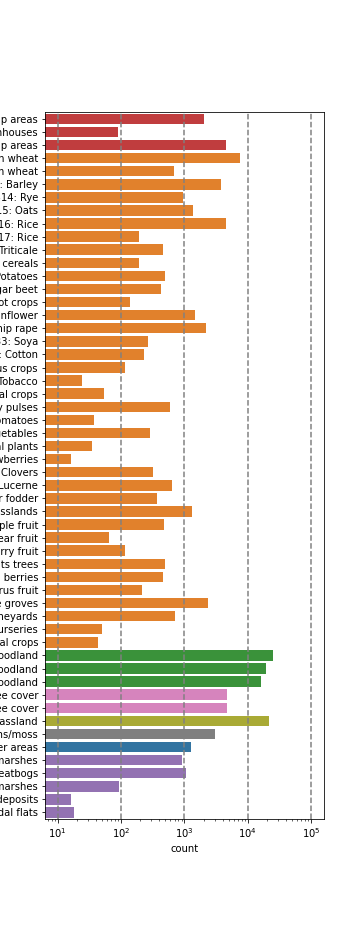
\includegraphics[width=\textwidth]{figs_05/fig_lucas_aoi_counts.png}
    \caption{Number of LUCAS points per LUCAS class used to validate the land cover maps, colored based on their level 1 class.}
    \label{fig:05_lucas_aoi_counts}
    \end{figure}

\subsection{Land Cover Modeling}

    The predicted probabilities on the calibration points were classified with both MPA and IMP on calibration points to assess their relative accuracy. Table \ref{tab:05_calibration_accuracy} shows that MPA produced the highest weighted precision at each level of the legend, while IMP produced the highest weighted F1-score by harmonizing precision and recall. The hierarchical confusion matrix in Figure~\ref{fig:05_confusion_matrix} shows that many crop types were frequently misclassified as \textit{Common Wheat}, \textit{Barley}, and \textit{Maize} within the textit{Cropland} level 1 class, while many cereal and fruit crops were frequently confused with \textit{Grassland}. 'Orchard' classes such as \textit{Apple fruit} and \textit{Pear fruit} orchards were also frequently confused with forest classes. The large non-hierarchical classes, Grassland, Bare Land, and Water, were among the most accurately classified, especially at level 3.
    
    \begin{table}[]
    \begin{tabular}{lrrrr}
    \textbf{Method} & \multicolumn{1}{l}{\textbf{Level}} & \multicolumn{1}{l}{\textbf{Precision}} & \multicolumn{1}{l}{\textbf{Recall}} & \multicolumn{1}{l}{\textbf{F1}} \\
    MPA & 1 & \textbf{0.76} & 0.70 & 0.69 \\
    MPA & 2 & 0.60 & 0.49 & 0.51 \\
    MPA & 3 & 0.59 & 0.45 & 0.48 \\
    IMP & 1 & 0.74 & \textbf{0.74} & \textbf{0.74} \\
    IMP & 2 & 0.57 & 0.57 & 0.57 \\
    IMP & 3 & 0.55 & 0.55 & 0.55
    \end{tabular}
    \caption{Weighted precision, recall and F1-score on calibration points at three levels in the LUCAS land cover hierarchy (8, 19, and 53 classes) by maximum probability assignment and iterative mapping of probabilities}
    \label{tab:05_calibration_accuracy}
    \end{table}

    \begin{table}[H!]
    \begin{tabular}{lrrrr}
    \textbf{Method} & \multicolumn{1}{l}{\textbf{Level}} & \multicolumn{1}{l}{\textbf{Precision}} & \multicolumn{1}{l}{\textbf{Recall}} & \multicolumn{1}{l}{\textbf{F1}} \\
    MPA & 1 & \textbf{0.66} & 0.57 & 0.58 \\
    MPA & 2 & 0.51 & 0.34 & 0.37 \\
    MPA & 3 & 0.47 & 0.29 & 0.33 \\
    IMP & 1 & 0.61 & \textbf{0.61} & \textbf{0.61} \\
    IMP & 2 & 0.43 & 0.43 & 0.43 \\
    IMP & 3 & 0.39 & 0.39 & 0.39
    \end{tabular}
    \caption{Weighted precision, recall and F1-score on LUCAS points at three levels in the LUCAS land cover hierarchy (8, 19, and 53 classes) by maximum probability assignment and iterative mapping of probabilities}
    \label{tab:05_calibration_accuracy}
    \end{table}

    \begin{figure}[H]
        \centering
        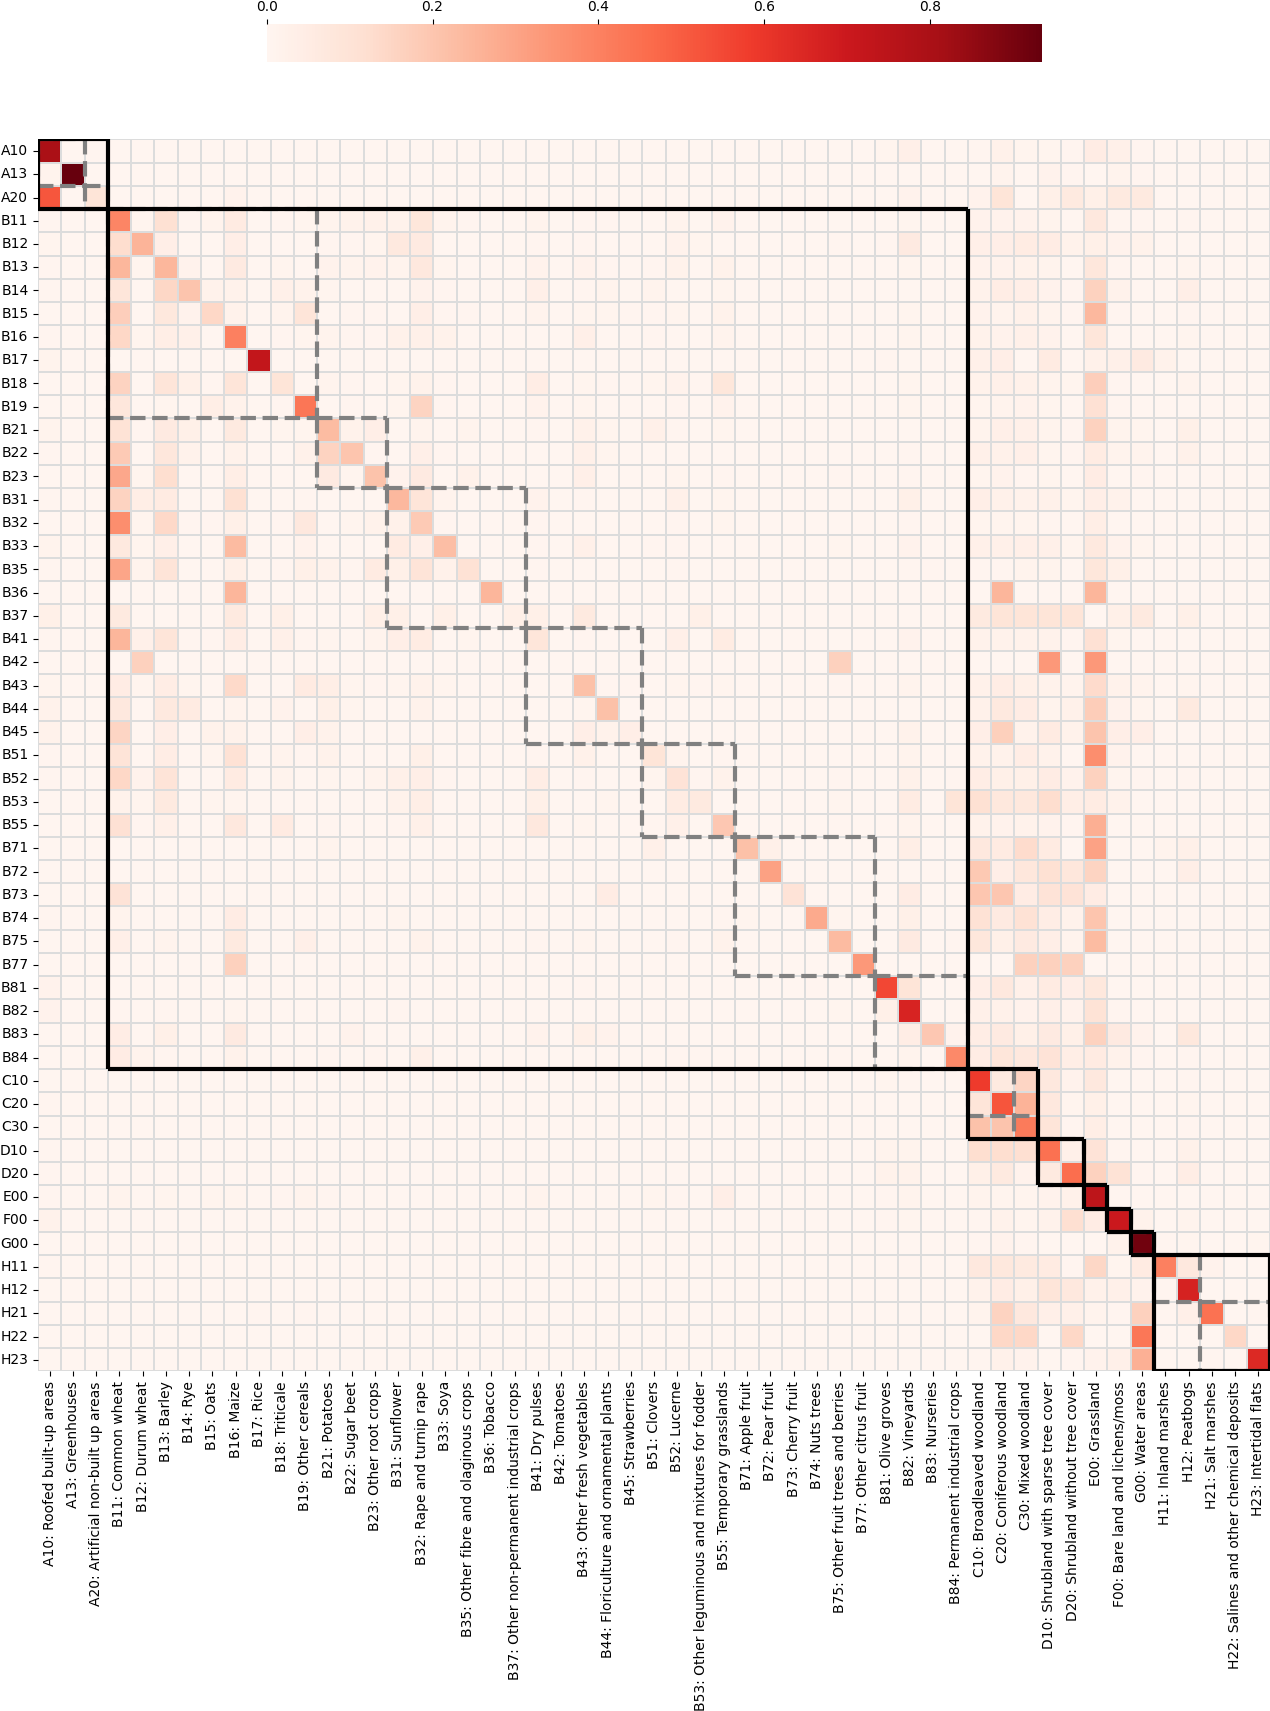
\includegraphics[width=\textwidth]{figs_05/fig_hierarchical_confusion_matrix_calib.png}
        \caption{Confusion matrix of the calibration points classified by IMP, normalized based on true class quantities. Red squares mean that the true class (x-axis) was often incorrectly predicted as the predicted class (y-axis)The grey dashed lines indicate which classes belong to the same level 2 class in the hierarchical legend. The black lines indicate level 1 class membership.}
        \label{fig:05_confusion_matrix_calib}
    \end{figure}

    \begin{figure}[H]
        \centering
        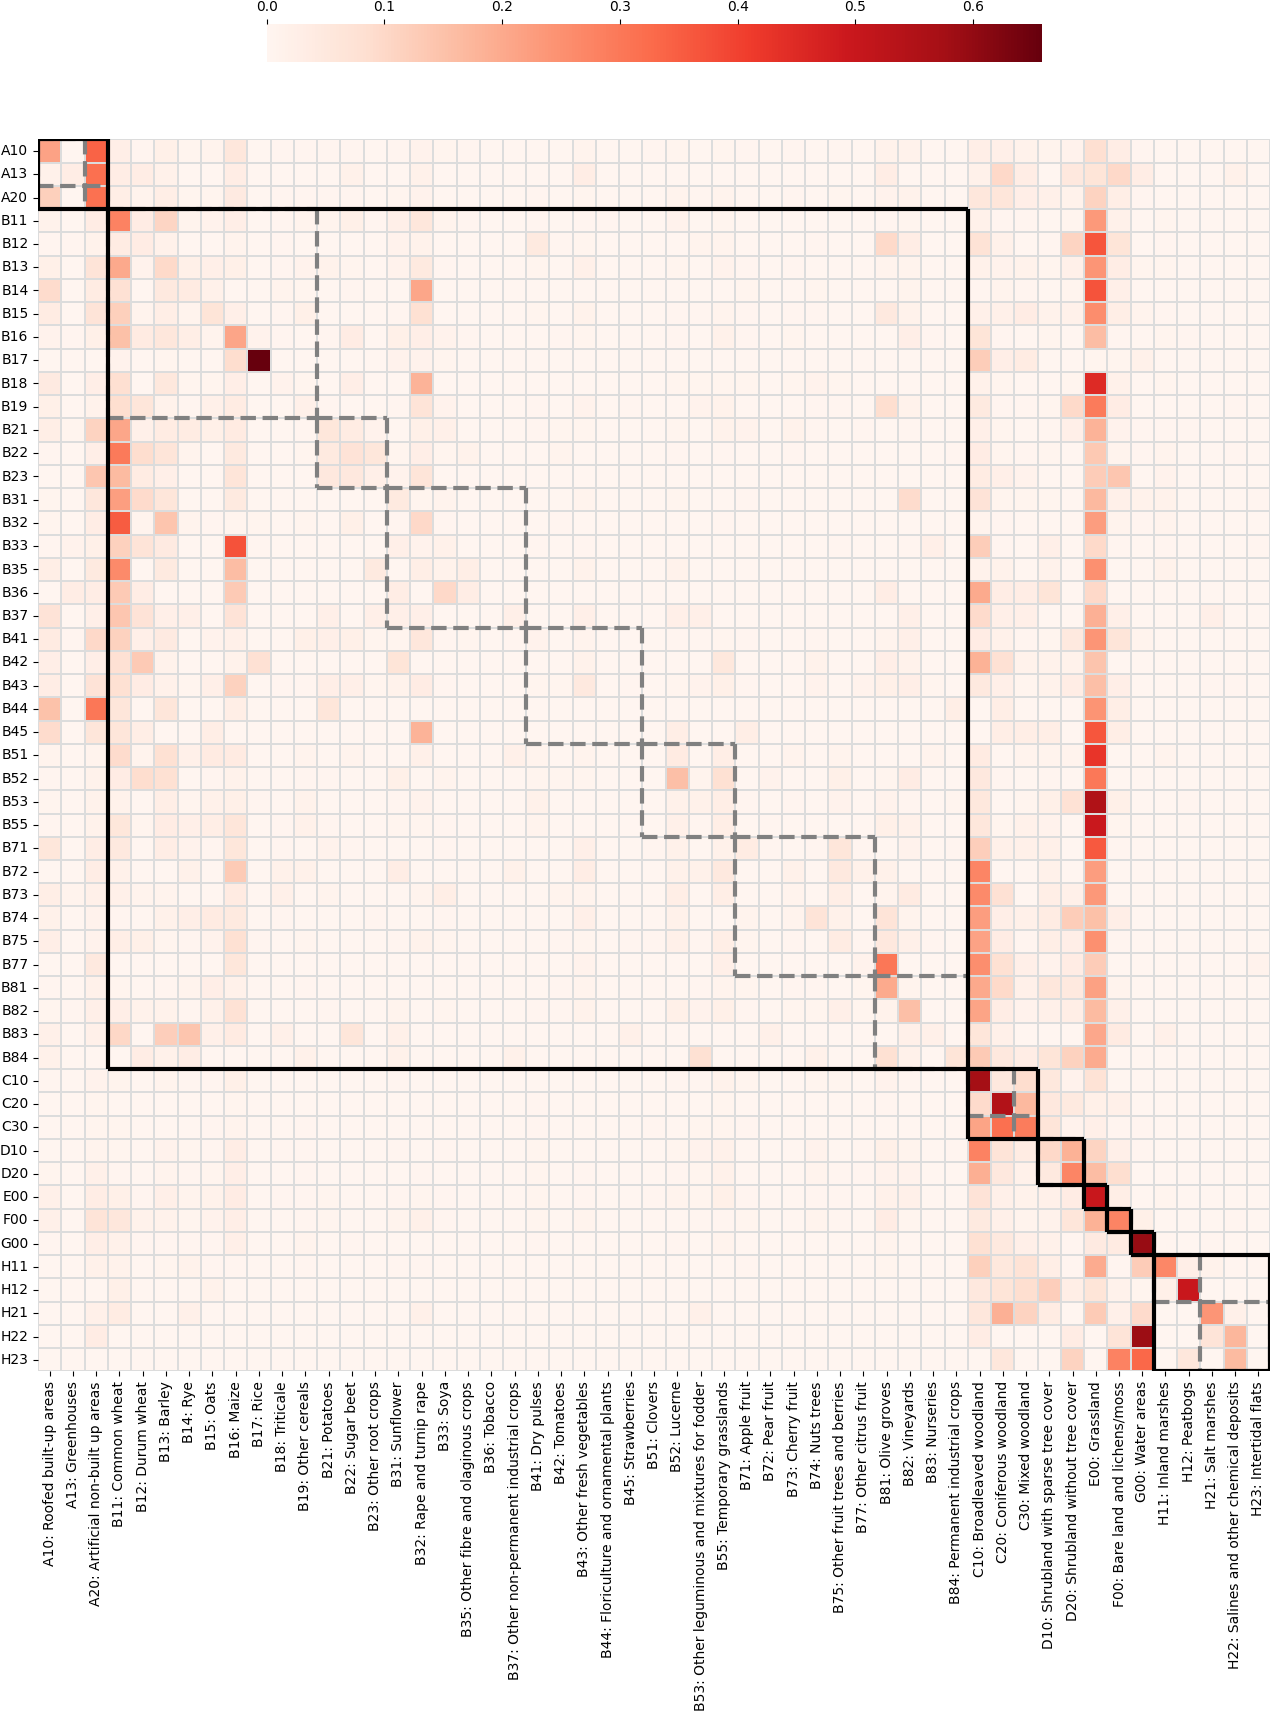
\includegraphics[width=\textwidth]{figs_05/fig_hierarchical_confusion_matrix_lucas.png}
        \caption{Confusion matrix of the LUCAS points classified by IMP, normalized based on true class quantities. Red squares mean that the true class (x-axis) was often incorrectly predicted as the predicted class (y-axis)The grey dashed lines indicate which classes belong to the same level 2 class in the hierarchical legend. The black lines indicate level 1 class membership.}
        \label{fig:05_confusion_matrix_lucas}
    \end{figure}

    \subsubsection{Spatiotemporal consistency}

        Table\@~\ref{tab:f1_space_time} compares the weighted F1-scores across the 51 different NUTS2 areas and 3 years. The accuracy of the model was more consistent through time than through space, with standard deviations across years being less than half the standard deviations across NUTS2 areas. Fig.\@~\ref{fig:f1_lucas_aoi} shows that areas farther away from France were classified less accurately, and Fig.\@~\ref{fig:boxplot_f1_year_lvl} shows that predictions on the 16 areas from 2015 were more consistent than the 7 areas in 2012 and the 29 areas in 2018.
        ref{fig:}

        \begin{table}[]
        \begin{tabular}{llll}
        Comparison & Level & Mean & Std \\
        Years & 1 & 0.562 & 0.071 \\
         & 2 & 0.372 & 0.045 \\
         & 3 & 0.317 & 0.040 \\
        NUTS2 areas & 1 & 0.590 & 0.176 \\
         & 2 & 0.386 & 0.181 \\
         & 3 & 0.332 & 0.187
        \end{tabular}
        \caption{Comparison of F1 consistency through time and space: Mean and standard deviation of F1-scores of testing model predictions on the LUCAS points from different NUTS2 areas and years. Note that the standard deviation across years is consistently less than half the standard deviation across NUTS2 areas.}
        \label{tab:f1_space_time}
        \end{table}
        
    \begin{figure}
    \begin{subfigure}[b]{width=0.48\linewidth}
        \centering
        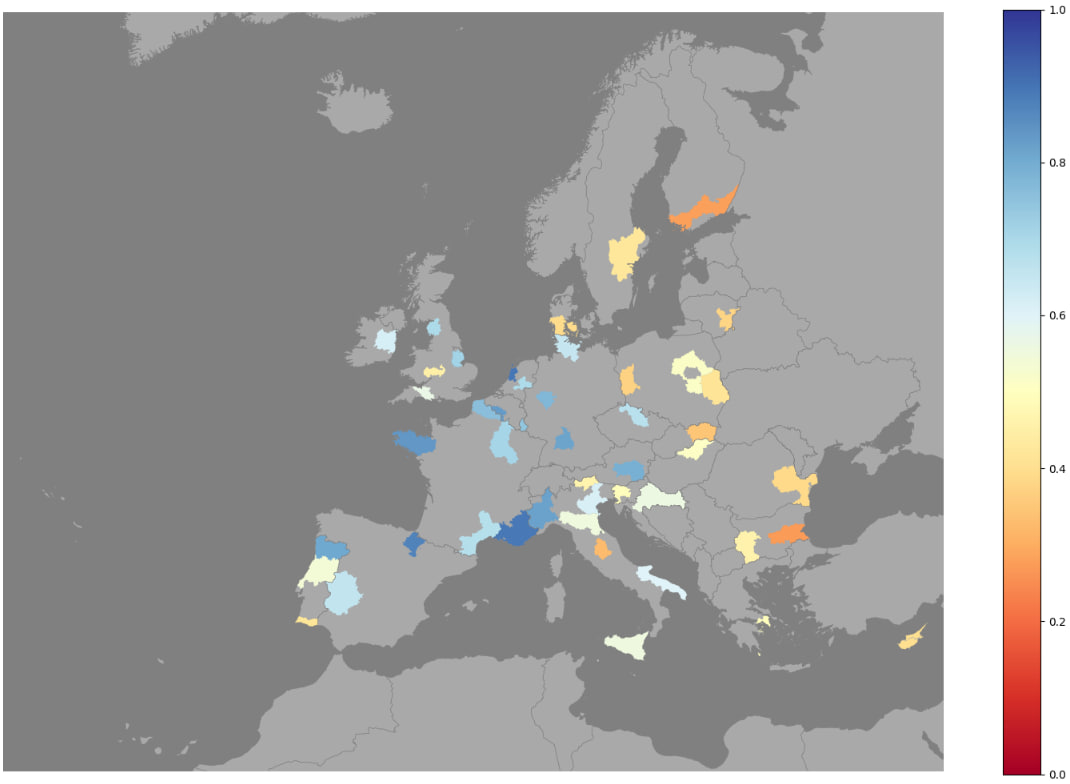
\includegraphics[width=1\linewidth]{figs_05/f1_lvl1.png}
        \caption{F1-score at level 1 (8 classes)}
        \label{fig:f1_lvl1}
    \end{subfigure}
    \hfill
    \begin{subfigure}[b]{width=0.48\linewidth}
        \centering
        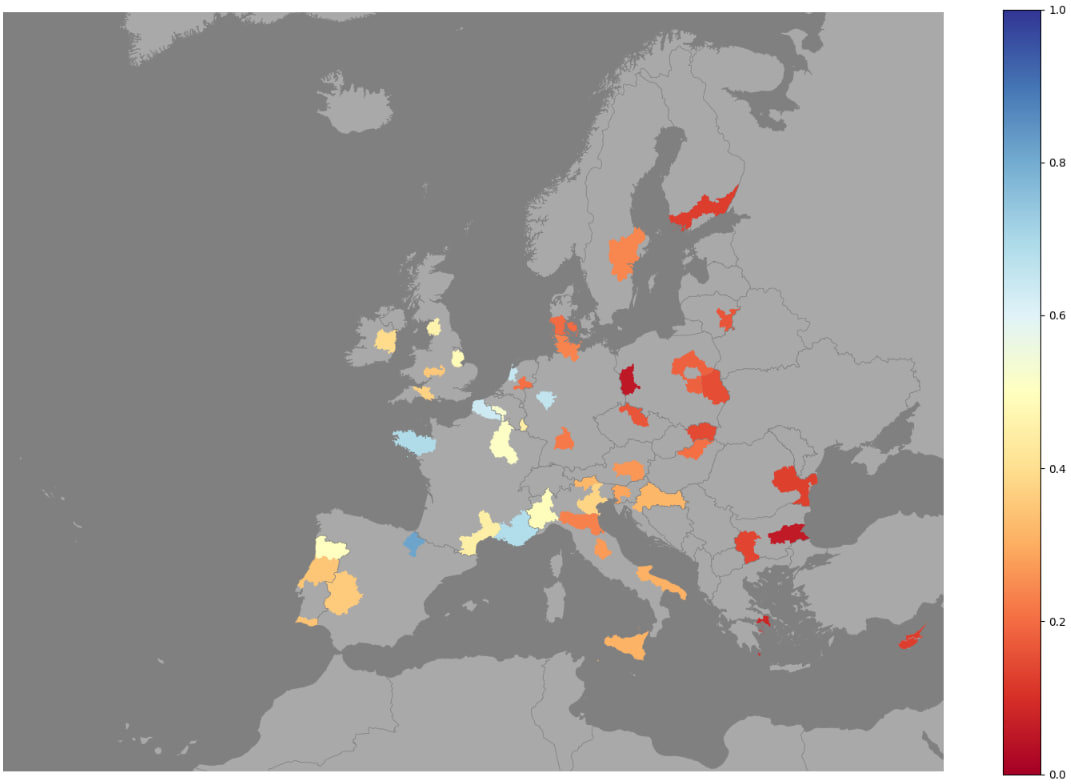
\includegraphics[width=1\linewidth]{figs_05/f1_lvl3.png}
        \caption{F1-score at level 3 (53 classes)}
        \label{fig:f1_lvl1}
    \end{subfigure}
    \ref{fig:f1_lucas_aoi}
    \caption{Comparison of F1-score across the different NUTS2 areas included in this study. Note that the areas in Eastern Europe were generally classified less accurately than those in Western Europe, and more specifically, near France.}
    \end{figure}

    \begin{figure}
        \centering
        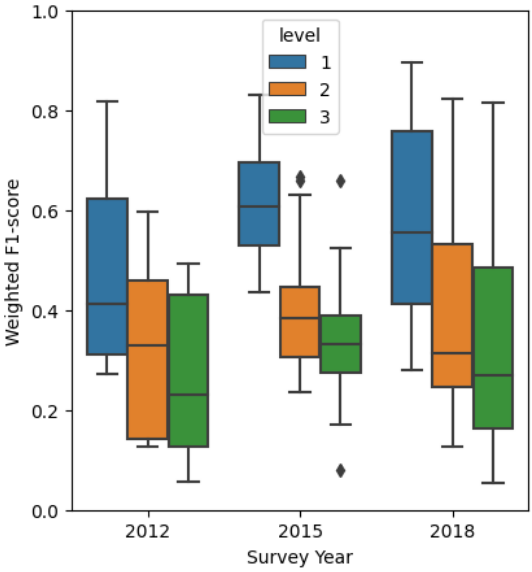
\includegraphics[width=0.5\linewidth]{figs_05/boxplot_f1_year_lvl.png}
        \caption{Boxplot of weighted F1-scores of all NUTS2/year combinations, separated by survey year and by legend level. Note that aggregating the predictions of 2015 to level 1 caused a relatively larger gain in accuracy than for 2012.}
        \label{fig:boxplot_f1_year_lvl}
    \end{figure}

    \subsection{Selective Hierarchical Classification}

        Figure~\ref{fig:05_comparison_metrics_calib} shows the highest predicted probability and the margin of victory for maximum probability classification, and the classification iteration for IMP.
        
        \begin{figure}
            \centering
            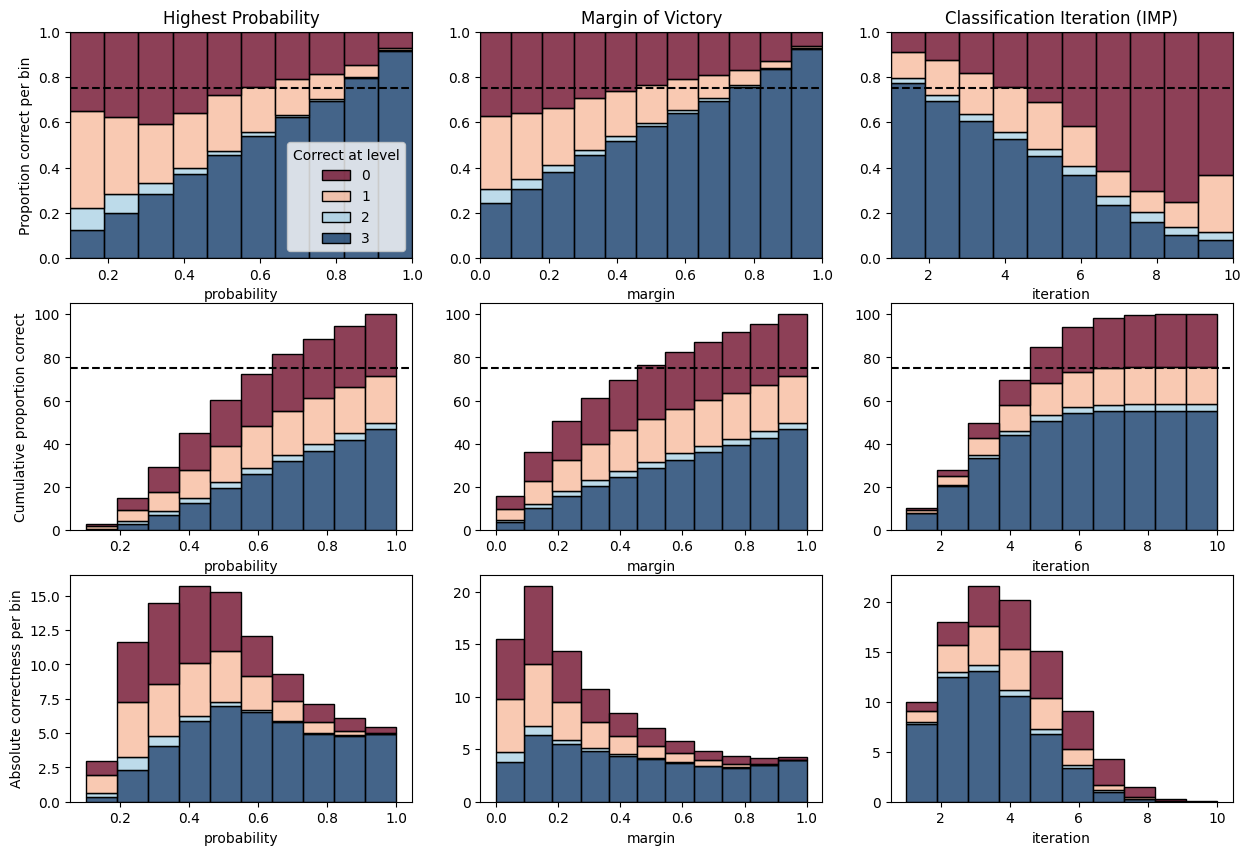
\includegraphics[width=\linewidth]{figs_05/fig_calibration_calib.png}
            \caption{Level of correctness of land cover classification on calibration points per level in the hierarchy in ten groups based on highest probability, margin of victory, and IMP classification iteration. 
            Blue indicates the predictions were correct at the third level of the legend; light blue that they were not correct at level 3 but were correct at level 2; the orange part indicates predictions that were only correct at level 1, and red indicates predictions that were completely incorrect.
            The top graphs show the proportion per group, the middle graphs show the cumulative correctness, and the bottom graphs show the amount of points that fall within each group.}
            \label{fig:05_comparison_metrics_calib}
        \end{figure}

         \begin{figure}
            \centering
            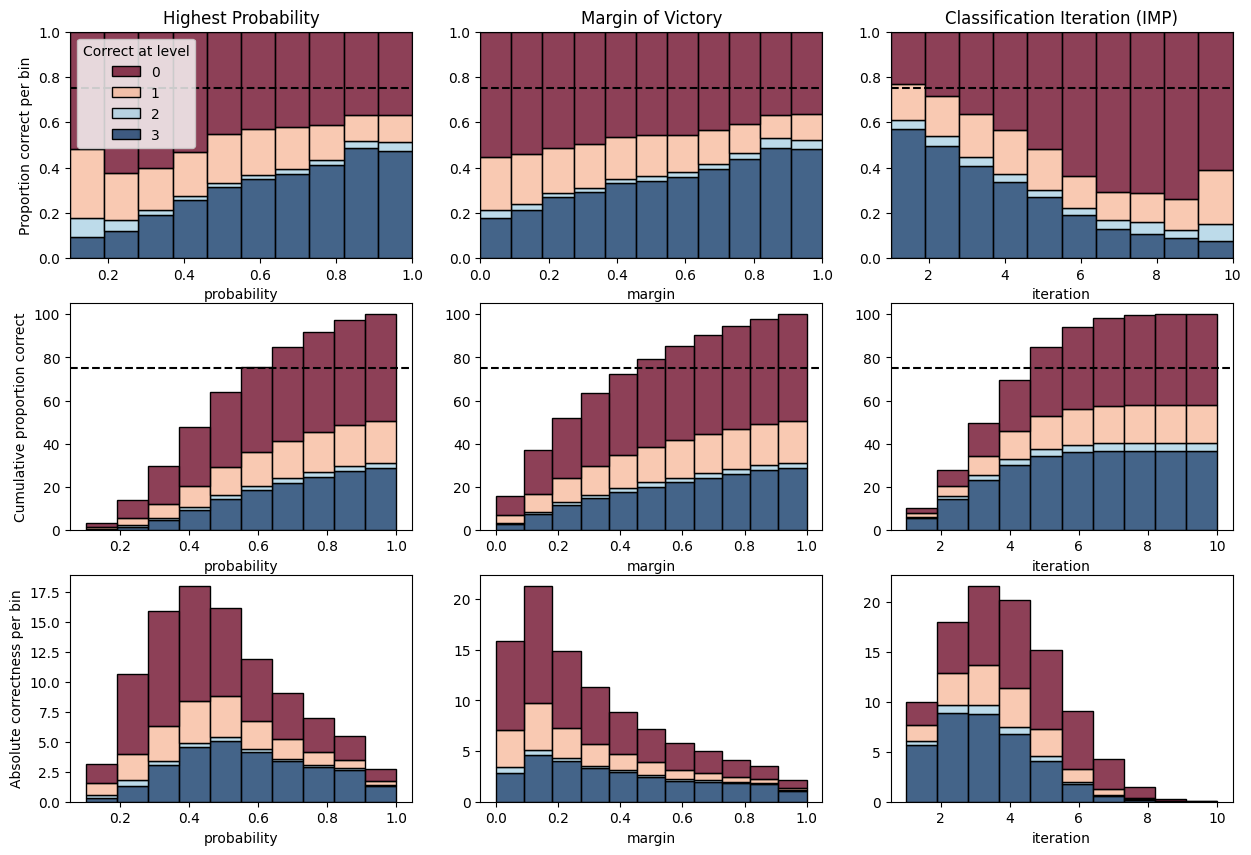
\includegraphics[width=\linewidth]{figs_05/fig_calibration_lucas.png}
            \caption{Level of correctness of land cover classification on LUCAS points per level in the hierarchy in ten groups based on highest probability, margin of victory, and IMP classification iteration. 
            Blue indicates the predictions were correct at the third level of the legend; light blue that they were not correct at level 3 but were correct at level 2; the orange part indicates predictions that were only correct at level 1, and red indicates predictions that were completely incorrect.
            The top graphs show the proportion per group, the middle graphs show the cumulative correctness, and the bottom graphs show the amount of points that fall within each group.}
            \label{fig:05_comparison_metrics_lucas}
        \end{figure}

\section{Discussion}

    % \subsection{How to use?}
    %     Selective hierarchical classification improves upon selective classification by maximizing the amount of pixels with information, and optimizing the balance between accuracy and detail. This gives researchers and policy-makers a better idea of what they 
    %     selective classification exists; it leaves parts empty. Is it better to have something than nothing?
    %     how to visualize these maps?
    %     how to use hierarchical maps in GIS software?
    %         help focus on areas that need to be studied/sampled better
    %     how to use their data?
    %         combine different level predictions into ensembles
        
    \subsection{Area estimates and model bias}

        When we applied IMP to classify the calibration points, we used the class proportion of the points themselves as a proxy for the area estimate. The resulting hard-class classification had identical precision and recall for each class. The class proportion of the calibration points can be considered a 'perfect' area estimate because it is a count, and not an estimation by statistics. \citet{witjes2024iterative} noted that precision and recall were more similar in IMP-produced hard class maps than in maximum probability assignment maps, but they were not identical, as in our calibration results in this work. The results from that work were based on area estimates from Eurostat, which have variance and are not perfectly accurate. This suggests that more accurate area estimates might result in proportional maps that have a closer class-wise link between precision and accuracy. If this is correct, IMP can be used to quantify how representative a validation dataset is of its study area.
    
    \subsection{Legend}
        We lost much detail in our legend because we needed 1) training data, 2) area estimates, and 3) validation points. We had training data for a lot of water \& bare land subclasses. It would be good if Eurostat made area estimates for all LUCAS land cover classes; we could have included them.

        It is also possible to omit using area estimates altogether and instead use the LUCAS class proportions directly. This would allow us to not only leverage the full 74-class LUCAS land cover legend, but also its land \textbf{use} legend. This would make it possible to separate grassland into pastures, natural grass, airport grassland, and many more classes. It would be more difficult to validate the proportionality of such maps without collaboration with Eurostat statisticians, however. 

        